\documentclass{book}
\usepackage[a4paper,top=2.5cm,bottom=2.5cm,left=2.5cm,right=2.5cm]{geometry}
\usepackage{makeidx}
\usepackage{natbib}
\usepackage{graphicx}
\usepackage{multicol}
\usepackage{float}
\usepackage{listings}
\usepackage{color}
\usepackage{ifthen}
\usepackage[table]{xcolor}
\usepackage{textcomp}
\usepackage{alltt}
\usepackage{ifpdf}
\ifpdf
\usepackage[pdftex,
            pagebackref=true,
            colorlinks=true,
            linkcolor=blue,
            unicode
           ]{hyperref}
\else
\usepackage[ps2pdf,
            pagebackref=true,
            colorlinks=true,
            linkcolor=blue,
            unicode
           ]{hyperref}
\usepackage{pspicture}
\fi
\usepackage[utf8]{inputenc}
\usepackage{mathptmx}
\usepackage[scaled=.90]{helvet}
\usepackage{courier}
\usepackage{sectsty}
\usepackage[titles]{tocloft}
\usepackage{doxygen}
\lstset{language=C++,inputencoding=utf8,basicstyle=\footnotesize,breaklines=true,breakatwhitespace=true,tabsize=8,numbers=left }
\makeindex
\setcounter{tocdepth}{3}
\renewcommand{\footrulewidth}{0.4pt}
\renewcommand{\familydefault}{\sfdefault}
\hfuzz=15pt
\setlength{\emergencystretch}{15pt}
\hbadness=750
\tolerance=750
\begin{document}
\hypersetup{pageanchor=false,citecolor=blue}
\begin{titlepage}
\vspace*{7cm}
\begin{center}
{\Large libap2p \\[1ex]\large 0.\-0.\-0 }\\
\vspace*{1cm}
{\large Generated by Doxygen 1.8.1}\\
\vspace*{0.5cm}
{\small Sat Jun 16 2012 17:37:24}\\
\end{center}
\end{titlepage}
\clearemptydoublepage
\pagenumbering{roman}
\tableofcontents
\clearemptydoublepage
\pagenumbering{arabic}
\hypersetup{pageanchor=true,citecolor=blue}
\chapter{Todo List}
\label{todo}
\hypertarget{todo}{}

\begin{DoxyRefList}
\item[\label{todo__todo000001}%
\hypertarget{todo__todo000001}{}%
Member \hyperlink{classlibap2p_1_1message_a9fbf46058138df50dff71e53d04ad383}{libap2p\-:\-:message\-:\-:get\-\_\-xml} ()]Stub, to complete! 
\end{DoxyRefList}
\chapter{Class Index}
\section{Class Hierarchy}
This inheritance list is sorted roughly, but not completely, alphabetically\-:\begin{DoxyCompactList}
\item \contentsline{section}{libap2p\-:\-:D\-H\-T}{\pageref{classlibap2p_1_1DHT}}{}
\item \contentsline{section}{libap2p\-:\-:dht\-\_\-entry}{\pageref{classlibap2p_1_1dht__entry}}{}
\item \contentsline{section}{libap2p\-:\-:message}{\pageref{classlibap2p_1_1message}}{}
\item \contentsline{section}{libap2p\-:\-:network}{\pageref{classlibap2p_1_1network}}{}
\item \contentsline{section}{libap2p\-:\-:node}{\pageref{classlibap2p_1_1node}}{}
\item \contentsline{section}{libap2p\-:\-:node\-\_\-connection}{\pageref{classlibap2p_1_1node__connection}}{}
\begin{DoxyCompactList}
\item \contentsline{section}{libap2p\-:\-:client\-\_\-node\-\_\-connection}{\pageref{classlibap2p_1_1client__node__connection}}{}
\item \contentsline{section}{libap2p\-:\-:server\-\_\-node\-\_\-connection}{\pageref{classlibap2p_1_1server__node__connection}}{}
\end{DoxyCompactList}
\end{DoxyCompactList}

\chapter{Class Index}
\section{Class List}
Here are the classes, structs, unions and interfaces with brief descriptions\-:\begin{DoxyCompactList}
\item\contentsline{section}{\hyperlink{classlibap2p_1_1client__node__connection}{libap2p\-::client\-\_\-node\-\_\-connection} }{\pageref{classlibap2p_1_1client__node__connection}}{}
\item\contentsline{section}{\hyperlink{classlibap2p_1_1DHT}{libap2p\-::\-D\-H\-T} }{\pageref{classlibap2p_1_1DHT}}{}
\item\contentsline{section}{\hyperlink{classlibap2p_1_1dht__entry}{libap2p\-::dht\-\_\-entry} }{\pageref{classlibap2p_1_1dht__entry}}{}
\item\contentsline{section}{\hyperlink{classlibap2p_1_1identity}{libap2p\-::identity} }{\pageref{classlibap2p_1_1identity}}{}
\item\contentsline{section}{\hyperlink{classlibap2p_1_1message}{libap2p\-::message} }{\pageref{classlibap2p_1_1message}}{}
\item\contentsline{section}{\hyperlink{classlibap2p_1_1network}{libap2p\-::network} }{\pageref{classlibap2p_1_1network}}{}
\item\contentsline{section}{\hyperlink{classlibap2p_1_1node}{libap2p\-::node} \\*\-:Represents a peer in the \hyperlink{classlibap2p_1_1network}{libap2p\-::network}. Used to send \hyperlink{classlibap2p_1_1message}{libap2p\-::message} objects, receiving them and other communication }{\pageref{classlibap2p_1_1node}}{}
\item\contentsline{section}{\hyperlink{classlibap2p_1_1node__connection}{libap2p\-::node\-\_\-connection} }{\pageref{classlibap2p_1_1node__connection}}{}
\item\contentsline{section}{\hyperlink{classlibap2p_1_1server}{libap2p\-::server} \\*\-: Main p2p listening class Internally called }{\pageref{classlibap2p_1_1server}}{}
\item\contentsline{section}{\hyperlink{classlibap2p_1_1server__node__connection}{libap2p\-::server\-\_\-node\-\_\-connection} \\*Implementation of listening \hyperlink{classlibap2p_1_1node__connection}{node\-\_\-connection} }{\pageref{classlibap2p_1_1server__node__connection}}{}
\end{DoxyCompactList}

\chapter{Class Documentation}
\hypertarget{classlibap2p_1_1client__node__connection}{\section{libap2p\-:\-:client\-\_\-node\-\_\-connection Class Reference}
\label{classlibap2p_1_1client__node__connection}\index{libap2p\-::client\-\_\-node\-\_\-connection@{libap2p\-::client\-\_\-node\-\_\-connection}}
}
Inheritance diagram for libap2p\-:\-:client\-\_\-node\-\_\-connection\-:\begin{figure}[H]
\begin{center}
\leavevmode
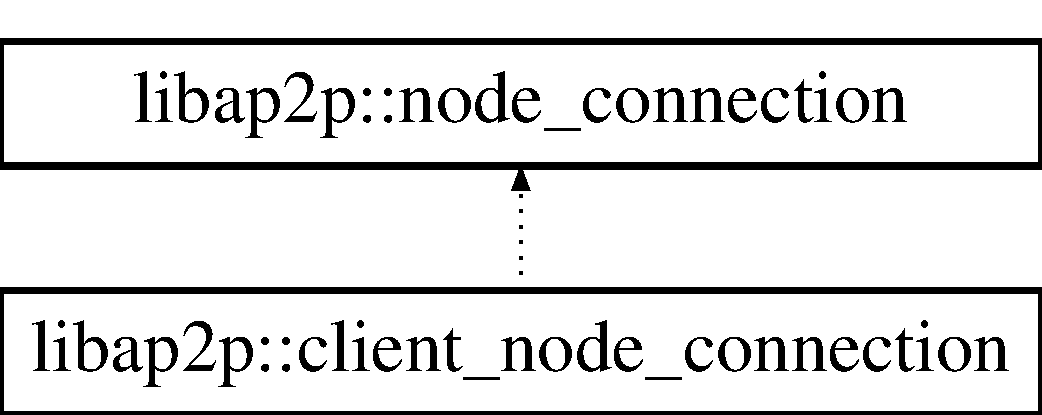
\includegraphics[height=2.000000cm]{classlibap2p_1_1client__node__connection}
\end{center}
\end{figure}
\subsection*{Public Member Functions}
\begin{DoxyCompactItemize}
\item 
\hypertarget{classlibap2p_1_1client__node__connection_a3e31f5b91ba46cb53521506d2a039293}{void {\bfseries send\-\_\-message} (\hyperlink{classlibap2p_1_1message}{message} $\ast$)}\label{classlibap2p_1_1client__node__connection_a3e31f5b91ba46cb53521506d2a039293}

\end{DoxyCompactItemize}


\subsection{Detailed Description}


Definition at line 30 of file client\-\_\-node\-\_\-connection.\-hpp.



The documentation for this class was generated from the following files\-:\begin{DoxyCompactItemize}
\item 
include/node/client\-\_\-node\-\_\-connection.\-hpp\item 
src/node/client\-\_\-node\-\_\-connection.\-cpp\end{DoxyCompactItemize}

\hypertarget{classlibap2p_1_1DHT}{\section{libap2p\-:\-:D\-H\-T Class Reference}
\label{classlibap2p_1_1DHT}\index{libap2p\-::\-D\-H\-T@{libap2p\-::\-D\-H\-T}}
}
\subsection*{Public Member Functions}
\begin{DoxyCompactItemize}
\item 
\hypertarget{classlibap2p_1_1DHT_a2be1b5d1723483db68c7f9d31307f354}{\hyperlink{classlibap2p_1_1dht__entry}{dht\-\_\-entry} $\ast$ {\bfseries fetch} ()}\label{classlibap2p_1_1DHT_a2be1b5d1723483db68c7f9d31307f354}

\end{DoxyCompactItemize}


\subsection{Detailed Description}


Definition at line 27 of file dht.\-hpp.



The documentation for this class was generated from the following file\-:\begin{DoxyCompactItemize}
\item 
include/\-D\-H\-T/dht.\-hpp\end{DoxyCompactItemize}

\hypertarget{classlibap2p_1_1dht__entry}{\section{libap2p\-:\-:dht\-\_\-entry Class Reference}
\label{classlibap2p_1_1dht__entry}\index{libap2p\-::dht\-\_\-entry@{libap2p\-::dht\-\_\-entry}}
}
\subsection*{Public Member Functions}
\begin{DoxyCompactItemize}
\item 
\hyperlink{classlibap2p_1_1dht__entry_a4bbb2a68e645b60d53af503979f2deb9}{dht\-\_\-entry} (std\-::string)
\begin{DoxyCompactList}\small\item\em Constructor. \end{DoxyCompactList}\end{DoxyCompactItemize}


\subsection{Detailed Description}


Definition at line 22 of file dht\-\_\-entry.\-hpp.



\subsection{Constructor \& Destructor Documentation}
\hypertarget{classlibap2p_1_1dht__entry_a4bbb2a68e645b60d53af503979f2deb9}{\index{libap2p\-::dht\-\_\-entry@{libap2p\-::dht\-\_\-entry}!dht\-\_\-entry@{dht\-\_\-entry}}
\index{dht\-\_\-entry@{dht\-\_\-entry}!libap2p::dht_entry@{libap2p\-::dht\-\_\-entry}}
\subsubsection[{dht\-\_\-entry}]{\setlength{\rightskip}{0pt plus 5cm}libap2p\-::dht\-\_\-entry\-::dht\-\_\-entry (
\begin{DoxyParamCaption}
\item[{std\-::string}]{filename}
\end{DoxyParamCaption}
)}}\label{classlibap2p_1_1dht__entry_a4bbb2a68e645b60d53af503979f2deb9}


Constructor. 


\begin{DoxyParams}{Parameters}
{\em std\-::string} & as local filename for \hyperlink{classlibap2p_1_1dht__entry}{dht\-\_\-entry} to load. \\
\hline
\end{DoxyParams}


Definition at line 28 of file dht\-\_\-entry.\-cpp.


\begin{DoxyCode}
\{
\}
\end{DoxyCode}


The documentation for this class was generated from the following files\-:\begin{DoxyCompactItemize}
\item 
include/\-D\-H\-T/dht\-\_\-entry.\-hpp\item 
src/\-D\-H\-T/dht\-\_\-entry.\-cpp\end{DoxyCompactItemize}

\hypertarget{classlibap2p_1_1identity}{\section{libap2p\-:\-:identity Class Reference}
\label{classlibap2p_1_1identity}\index{libap2p\-::identity@{libap2p\-::identity}}
}


\subsection{Detailed Description}


Definition at line 23 of file identity.\-hpp.



The documentation for this class was generated from the following files\-:\begin{DoxyCompactItemize}
\item 
include/identity/identity.\-hpp\item 
src/identity/identity.\-cpp\end{DoxyCompactItemize}

\hypertarget{classlibap2p_1_1message}{\section{libap2p\-:\-:message Class Reference}
\label{classlibap2p_1_1message}\index{libap2p\-::message@{libap2p\-::message}}
}
\subsection*{Public Member Functions}
\begin{DoxyCompactItemize}
\item 
\hypertarget{classlibap2p_1_1message_a433fa67765f72a86c6a022aa35ff06b7}{\hyperlink{classlibap2p_1_1message_a433fa67765f72a86c6a022aa35ff06b7}{message} ()}\label{classlibap2p_1_1message_a433fa67765f72a86c6a022aa35ff06b7}

\begin{DoxyCompactList}\small\item\em Default constructor. \end{DoxyCompactList}\item 
\hyperlink{classlibap2p_1_1message_a6609bf74f5cc5e2ea353751abcff149a}{message} (unsigned int, std\-::string)
\begin{DoxyCompactList}\small\item\em Constructor with data. Used to prepare a message to be send. \end{DoxyCompactList}\item 
\hyperlink{classlibap2p_1_1message_ab1c39ec5721f3520eed6735df2f335ef}{message} (std\-::string)
\begin{DoxyCompactList}\small\item\em Constructor from X\-M\-L content. \end{DoxyCompactList}\item 
std\-::string \hyperlink{classlibap2p_1_1message_a9fbf46058138df50dff71e53d04ad383}{get\-\_\-xml} ()
\begin{DoxyCompactList}\small\item\em Get the xml text for the message Internally used. \end{DoxyCompactList}\end{DoxyCompactItemize}


\subsection{Detailed Description}


Definition at line 27 of file message.\-hpp.



\subsection{Constructor \& Destructor Documentation}
\hypertarget{classlibap2p_1_1message_a6609bf74f5cc5e2ea353751abcff149a}{\index{libap2p\-::message@{libap2p\-::message}!message@{message}}
\index{message@{message}!libap2p::message@{libap2p\-::message}}
\subsubsection[{message}]{\setlength{\rightskip}{0pt plus 5cm}libap2p\-::message\-::message (
\begin{DoxyParamCaption}
\item[{unsigned int}]{messagetype, }
\item[{std\-::string}]{messagedata}
\end{DoxyParamCaption}
)}}\label{classlibap2p_1_1message_a6609bf74f5cc5e2ea353751abcff149a}


Constructor with data. Used to prepare a message to be send. 


\begin{DoxyParams}{Parameters}
{\em messagetype} & Message type. Can be any uint. Will be send through the socket \\
\hline
{\em messagedata} & The data to send. Easy construction by boost\-::asio\-::buffer(\mbox{[}anything here\mbox{]}); \\
\hline
\end{DoxyParams}


Definition at line 44 of file message.\-cpp.


\begin{DoxyCode}
\{
        this->\_init();
        this->\_message\_type = messagetype;
        this->\_message\_data = messagedata;
\}
\end{DoxyCode}
\hypertarget{classlibap2p_1_1message_ab1c39ec5721f3520eed6735df2f335ef}{\index{libap2p\-::message@{libap2p\-::message}!message@{message}}
\index{message@{message}!libap2p::message@{libap2p\-::message}}
\subsubsection[{message}]{\setlength{\rightskip}{0pt plus 5cm}libap2p\-::message\-::message (
\begin{DoxyParamCaption}
\item[{std\-::string}]{xml\-\_\-str}
\end{DoxyParamCaption}
)}}\label{classlibap2p_1_1message_ab1c39ec5721f3520eed6735df2f335ef}


Constructor from X\-M\-L content. 


\begin{DoxyParams}{Parameters}
{\em xml\-\_\-str} & an std\-::string with xml contents. \\
\hline
\end{DoxyParams}


Definition at line 55 of file message.\-cpp.


\begin{DoxyCode}
\{
        this->\_init();

        std::stringstream in;
        in << xml\_str;

        boost::property\_tree::ptree pt;

        read\_xml(in, pt);

        this->\_message\_version = pt.get<std::string>(\textcolor{stringliteral}{"libap2p.version"});
        this->\_message\_data = pt.get<std::string>(\textcolor{stringliteral}{"libap2p.message.data"});
        this->\_message\_type = pt.get<\textcolor{keywordtype}{unsigned} \textcolor{keywordtype}{int}>(\textcolor{stringliteral}{"libap2p.message.type"});
        this->\_message\_signature = pt.get<std::string>(\textcolor{stringliteral}{"
      libap2p.signature.signature"});
        this->\_message\_signature\_type = pt.get<std::string>(\textcolor{stringliteral}{"
      libap2p.signature.type"});
\}
\end{DoxyCode}


\subsection{Member Function Documentation}
\hypertarget{classlibap2p_1_1message_a9fbf46058138df50dff71e53d04ad383}{\index{libap2p\-::message@{libap2p\-::message}!get\-\_\-xml@{get\-\_\-xml}}
\index{get\-\_\-xml@{get\-\_\-xml}!libap2p::message@{libap2p\-::message}}
\subsubsection[{get\-\_\-xml}]{\setlength{\rightskip}{0pt plus 5cm}std\-::string libap2p\-::message\-::get\-\_\-xml (
\begin{DoxyParamCaption}
{}
\end{DoxyParamCaption}
)}}\label{classlibap2p_1_1message_a9fbf46058138df50dff71e53d04ad383}


Get the xml text for the message Internally used. 

\begin{DoxyReturn}{Returns}
The xml-\/structure of the message. 
\end{DoxyReturn}
todo\-: Check signature before sending? 

Definition at line 86 of file message.\-cpp.


\begin{DoxyCode}
\{
        boost::property\_tree::ptree pt;
        std::stringstream out;

        pt.put(\textcolor{stringliteral}{"libap2p.version"}, \textcolor{stringliteral}{"0.0.1"});
        pt.put(\textcolor{stringliteral}{"libap2p.message.type"}, this->\_message\_type);
        pt.put(\textcolor{stringliteral}{"libap2p.message.data"}, this->\_message\_data);
        pt.put(\textcolor{stringliteral}{"libap2p.signature.signature"}, this->\_message\_signature); 
        pt.put(\textcolor{stringliteral}{"libap2p.signature.type"}, this->\_message\_signature\_type);
        
        write\_xml(out, pt);
        
        \textcolor{keywordflow}{return} out.str();
\}
\end{DoxyCode}


The documentation for this class was generated from the following files\-:\begin{DoxyCompactItemize}
\item 
include/message/message.\-hpp\item 
src/message/message.\-cpp\end{DoxyCompactItemize}

\hypertarget{classlibap2p_1_1network}{\section{libap2p\-:\-:network Class Reference}
\label{classlibap2p_1_1network}\index{libap2p\-::network@{libap2p\-::network}}
}


{\ttfamily \#include $<$network.\-hpp$>$}

\subsection*{Public Member Functions}
\begin{DoxyCompactItemize}
\item 
\hyperlink{classlibap2p_1_1network_a8ddd2d62c50c2ab85cb1ab884847748e}{network} ()
\item 
void \hyperlink{classlibap2p_1_1network_a0cf3ffa14a7fbad863b3db1d07382353}{connect} ()
\item 
void \hyperlink{classlibap2p_1_1network_a256421d58621e89fbf15a3cdc3f91ae6}{close} ()
\item 
\hypertarget{classlibap2p_1_1network_a721b9df35da2eb2797bd2262e5525b14}{void {\bfseries add\-\_\-node} (\hyperlink{classlibap2p_1_1node}{node} $\ast$)}\label{classlibap2p_1_1network_a721b9df35da2eb2797bd2262e5525b14}

\item 
connection\-\_\-status \hyperlink{classlibap2p_1_1network_aa01d40a45f84bb50a8210673e2a6b454}{status} () const 
\end{DoxyCompactItemize}


\subsection{Detailed Description}
The main class which gives access to the whole network. 

Definition at line 30 of file network.\-hpp.



\subsection{Constructor \& Destructor Documentation}
\hypertarget{classlibap2p_1_1network_a8ddd2d62c50c2ab85cb1ab884847748e}{\index{libap2p\-::network@{libap2p\-::network}!network@{network}}
\index{network@{network}!libap2p::network@{libap2p\-::network}}
\subsubsection[{network}]{\setlength{\rightskip}{0pt plus 5cm}libap2p\-::network\-::network (
\begin{DoxyParamCaption}
{}
\end{DoxyParamCaption}
)}}\label{classlibap2p_1_1network_a8ddd2d62c50c2ab85cb1ab884847748e}
Constructor. Initializes network structure 

Definition at line 27 of file network.\-cpp.


\begin{DoxyCode}
\{
        this->\_connection\_status = DISCONNECTED;
\}
\end{DoxyCode}


\subsection{Member Function Documentation}
\hypertarget{classlibap2p_1_1network_a256421d58621e89fbf15a3cdc3f91ae6}{\index{libap2p\-::network@{libap2p\-::network}!close@{close}}
\index{close@{close}!libap2p::network@{libap2p\-::network}}
\subsubsection[{close}]{\setlength{\rightskip}{0pt plus 5cm}void libap2p\-::network\-::close (
\begin{DoxyParamCaption}
{}
\end{DoxyParamCaption}
)}}\label{classlibap2p_1_1network_a256421d58621e89fbf15a3cdc3f91ae6}
Function to close the network. Whenever the connection should be closed, this is to be called. 

Definition at line 44 of file network.\-cpp.


\begin{DoxyCode}
\{
        this->\_connection\_status = DISCONNECTED;
\}
\end{DoxyCode}
\hypertarget{classlibap2p_1_1network_a0cf3ffa14a7fbad863b3db1d07382353}{\index{libap2p\-::network@{libap2p\-::network}!connect@{connect}}
\index{connect@{connect}!libap2p::network@{libap2p\-::network}}
\subsubsection[{connect}]{\setlength{\rightskip}{0pt plus 5cm}void libap2p\-::network\-::connect (
\begin{DoxyParamCaption}
{}
\end{DoxyParamCaption}
)}}\label{classlibap2p_1_1network_a0cf3ffa14a7fbad863b3db1d07382353}
Called to connect to the ap2p network. When called, ap2p connects to other nodes specified with add\-\_\-node() and fetches more from them. It will async build up connections. The progress can be followed in \hyperlink{classlibap2p_1_1network_aa01d40a45f84bb50a8210673e2a6b454}{network\-::status}. \begin{DoxyWarning}{Warning}
An initial node is to be added with add\-\_\-node or new network is created 
\end{DoxyWarning}


Definition at line 36 of file network.\-cpp.


\begin{DoxyCode}
\{
        this->\_connection\_status = CONNECTING;
\}
\end{DoxyCode}
\hypertarget{classlibap2p_1_1network_aa01d40a45f84bb50a8210673e2a6b454}{\index{libap2p\-::network@{libap2p\-::network}!status@{status}}
\index{status@{status}!libap2p::network@{libap2p\-::network}}
\subsubsection[{status}]{\setlength{\rightskip}{0pt plus 5cm}connection\-\_\-status libap2p\-::network\-::status (
\begin{DoxyParamCaption}
{}
\end{DoxyParamCaption}
) const\hspace{0.3cm}{\ttfamily [inline]}}}\label{classlibap2p_1_1network_aa01d40a45f84bb50a8210673e2a6b454}
Used to check the current connection status. Can be libap2p\{connection\-\_\-status \{C\-O\-N\-N\-E\-C\-T\-E\-D, C\-O\-N\-N\-E\-C\-T\-I\-N\-G, D\-I\-S\-C\-O\-N\-N\-E\-C\-T\-E\-D or E\-R\-R\-O\-R\}\}; 

Definition at line 42 of file network.\-hpp.


\begin{DoxyCode}
\{\textcolor{keywordflow}{return} this->\_connection\_status;\};
\end{DoxyCode}


The documentation for this class was generated from the following files\-:\begin{DoxyCompactItemize}
\item 
include/network/network.\-hpp\item 
src/network/network.\-cpp\end{DoxyCompactItemize}

\hypertarget{classlibap2p_1_1node}{\section{libap2p\-:\-:node Class Reference}
\label{classlibap2p_1_1node}\index{libap2p\-::node@{libap2p\-::node}}
}


\-:Represents a peer in the \hyperlink{classlibap2p_1_1network}{libap2p\-::network}. Used to send \hyperlink{classlibap2p_1_1message}{libap2p\-::message} objects, receiving them and other communication.  




{\ttfamily \#include $<$node.\-hpp$>$}

\subsection*{Public Member Functions}
\begin{DoxyCompactItemize}
\item 
\hypertarget{classlibap2p_1_1node_ae75928811247397aa11c692ead20e6ec}{\hyperlink{classlibap2p_1_1node_ae75928811247397aa11c692ead20e6ec}{node} ()}\label{classlibap2p_1_1node_ae75928811247397aa11c692ead20e6ec}

\begin{DoxyCompactList}\small\item\em \-: Constructor. Initializes node object \end{DoxyCompactList}\item 
\hypertarget{classlibap2p_1_1node_abc5bc4f3e11a2110156cdbcf21f92355}{{\bfseries node} (\hyperlink{classlibap2p_1_1node__connection}{node\-\_\-connection} $\ast$)}\label{classlibap2p_1_1node_abc5bc4f3e11a2110156cdbcf21f92355}

\item 
bool \hyperlink{classlibap2p_1_1node_acaab6b50b4a46a99b53c5e4bb2e78760}{connect} ()
\item 
void \hyperlink{classlibap2p_1_1node_a8601f7559082dc14f395b6cb6bbb5f0e}{send\-\_\-message} (\hyperlink{classlibap2p_1_1message}{message} $\ast$)
\begin{DoxyCompactList}\small\item\em \-: Send a \hyperlink{classlibap2p_1_1message}{libap2p\-::message} object to another node \end{DoxyCompactList}\end{DoxyCompactItemize}


\subsection{Detailed Description}
\-:Represents a peer in the \hyperlink{classlibap2p_1_1network}{libap2p\-::network}. Used to send \hyperlink{classlibap2p_1_1message}{libap2p\-::message} objects, receiving them and other communication. 

Definition at line 36 of file node.\-hpp.



\subsection{Member Function Documentation}
\hypertarget{classlibap2p_1_1node_acaab6b50b4a46a99b53c5e4bb2e78760}{\index{libap2p\-::node@{libap2p\-::node}!connect@{connect}}
\index{connect@{connect}!libap2p::node@{libap2p\-::node}}
\subsubsection[{connect}]{\setlength{\rightskip}{0pt plus 5cm}bool libap2p\-::node\-::connect (
\begin{DoxyParamCaption}
{}
\end{DoxyParamCaption}
)}}\label{classlibap2p_1_1node_acaab6b50b4a46a99b53c5e4bb2e78760}
\begin{DoxyRefDesc}{Todo}
\item[\hyperlink{todo__todo000001}{Todo}]\-: insert connection stuff here. \end{DoxyRefDesc}


Definition at line 35 of file node.\-cpp.


\begin{DoxyCode}
\{
        \textcolor{keywordflow}{return} \textcolor{keyword}{false}; \textcolor{comment}{//stub}
\}
\end{DoxyCode}
\hypertarget{classlibap2p_1_1node_a8601f7559082dc14f395b6cb6bbb5f0e}{\index{libap2p\-::node@{libap2p\-::node}!send\-\_\-message@{send\-\_\-message}}
\index{send\-\_\-message@{send\-\_\-message}!libap2p::node@{libap2p\-::node}}
\subsubsection[{send\-\_\-message}]{\setlength{\rightskip}{0pt plus 5cm}void libap2p\-::node\-::send\-\_\-message (
\begin{DoxyParamCaption}
\item[{{\bf message} $\ast$}]{msg}
\end{DoxyParamCaption}
)}}\label{classlibap2p_1_1node_a8601f7559082dc14f395b6cb6bbb5f0e}


\-: Send a \hyperlink{classlibap2p_1_1message}{libap2p\-::message} object to another node 


\begin{DoxyExceptions}{Exceptions}
{\em } & \\
\hline
\end{DoxyExceptions}


Definition at line 45 of file node.\-cpp.


\begin{DoxyCode}
\{
        \textcolor{keywordflow}{if}(this->\hyperlink{classlibap2p_1_1node_acaab6b50b4a46a99b53c5e4bb2e78760}{connect}())
        \{
                
        \}
        
\}
\end{DoxyCode}


The documentation for this class was generated from the following files\-:\begin{DoxyCompactItemize}
\item 
include/node/node.\-hpp\item 
src/node/node.\-cpp\end{DoxyCompactItemize}

\hypertarget{classlibap2p_1_1node__connection}{\section{libap2p\-:\-:node\-\_\-connection Class Reference}
\label{classlibap2p_1_1node__connection}\index{libap2p\-::node\-\_\-connection@{libap2p\-::node\-\_\-connection}}
}


{\ttfamily \#include $<$node\-\_\-connection.\-hpp$>$}

Inheritance diagram for libap2p\-:\-:node\-\_\-connection\-:\begin{figure}[H]
\begin{center}
\leavevmode
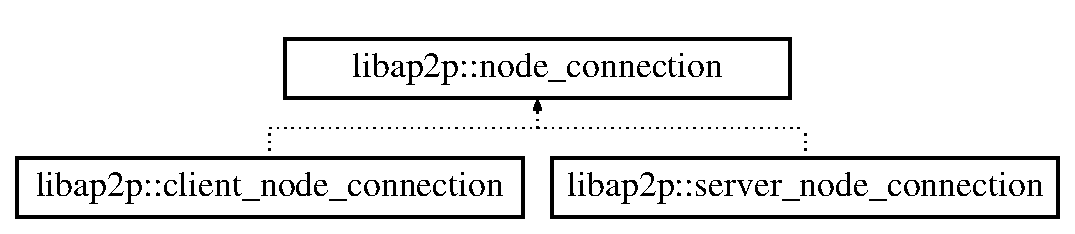
\includegraphics[height=2.000000cm]{classlibap2p_1_1node__connection}
\end{center}
\end{figure}


\subsection{Detailed Description}
Abstract class providing the connection with a node. Implemented by \hyperlink{classlibap2p_1_1server__node__connection}{server\-\_\-node\-\_\-connection} or \hyperlink{classlibap2p_1_1client__node__connection}{client\-\_\-node\-\_\-connection}. 

Definition at line 28 of file node\-\_\-connection.\-hpp.



The documentation for this class was generated from the following file\-:\begin{DoxyCompactItemize}
\item 
include/network/node\-\_\-connection.\-hpp\end{DoxyCompactItemize}

\hypertarget{classlibap2p_1_1server}{\section{libap2p\-:\-:server Class Reference}
\label{classlibap2p_1_1server}\index{libap2p\-::server@{libap2p\-::server}}
}


\-: Main p2p listening class Internally called.  




{\ttfamily \#include $<$server.\-hpp$>$}

\subsection*{Public Member Functions}
\begin{DoxyCompactItemize}
\item 
\hypertarget{classlibap2p_1_1server_a827f2a4dcc2f53e8113bb933afa477c3}{{\bfseries server} (\hyperlink{classlibap2p_1_1network}{libap2p\-::network} $\ast$, unsigned short)}\label{classlibap2p_1_1server_a827f2a4dcc2f53e8113bb933afa477c3}

\item 
\hypertarget{classlibap2p_1_1server_aa096494c1d08efd749ac6244dc271596}{void {\bfseries run} ()}\label{classlibap2p_1_1server_aa096494c1d08efd749ac6244dc271596}

\end{DoxyCompactItemize}


\subsection{Detailed Description}
\-: Main p2p listening class Internally called. 

Definition at line 31 of file server.\-hpp.



The documentation for this class was generated from the following files\-:\begin{DoxyCompactItemize}
\item 
include/network/server.\-hpp\item 
src/network/server.\-cpp\end{DoxyCompactItemize}

\hypertarget{classlibap2p_1_1server__node__connection}{\section{libap2p\-:\-:server\-\_\-node\-\_\-connection Class Reference}
\label{classlibap2p_1_1server__node__connection}\index{libap2p\-::server\-\_\-node\-\_\-connection@{libap2p\-::server\-\_\-node\-\_\-connection}}
}


{\ttfamily \#include $<$server\-\_\-node\-\_\-connection.\-hpp$>$}

Inheritance diagram for libap2p\-:\-:server\-\_\-node\-\_\-connection\-:\begin{figure}[H]
\begin{center}
\leavevmode
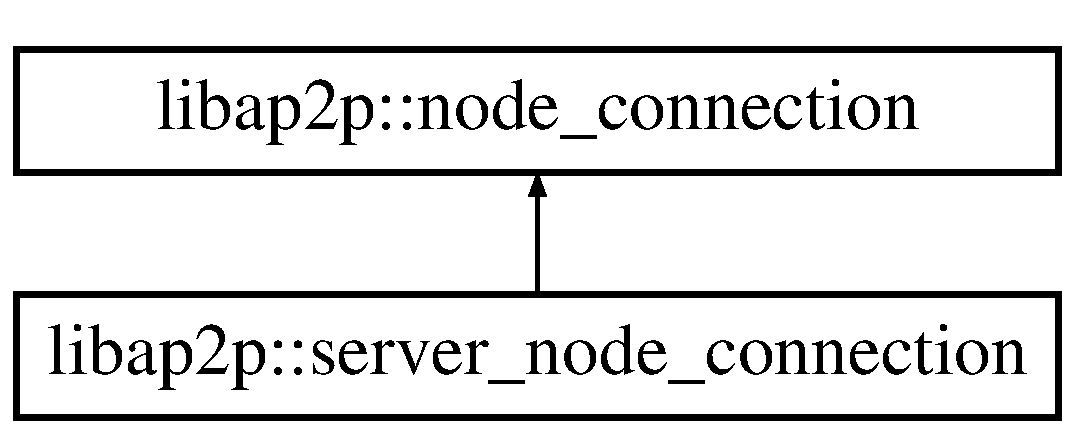
\includegraphics[height=2.000000cm]{classlibap2p_1_1server__node__connection}
\end{center}
\end{figure}


\subsection{Detailed Description}
Implementation of listening \hyperlink{classlibap2p_1_1node__connection}{node\-\_\-connection}. 

Definition at line 31 of file server\-\_\-node\-\_\-connection.\-hpp.



The documentation for this class was generated from the following files\-:\begin{DoxyCompactItemize}
\item 
include/network/server\-\_\-node\-\_\-connection.\-hpp\item 
src/network/server\-\_\-node\-\_\-connection.\-cpp\end{DoxyCompactItemize}

\printindex
\end{document}
